\documentclass[11pt,a4paper]{amsart}
\usepackage{setspace}
\doublespacing
\usepackage{amssymb,latexsym}
\usepackage{graphicx}
\theoremstyle{plain}
\newtheorem{theorem}{Theorem}
\newtheorem{corollary}{Corollary}
\newtheorem{lemma}{Lemma}
\newtheorem{axiom}{Axiom}
\newtheorem{proposition}{Proposition}
\usepackage{geometry}
\geometry{a4paper,left=2cm,right=2cm,top=1cm,bottom=1cm}
\theoremstyle{definition}
\newtheorem{definition}{Definition}
\usepackage{ulem} % various underlines
\usepackage{hyperref} % to insert URL 
\usepackage{graphicx} % to insert illustration
\usepackage[mathscr]{eucal} % to express a collection of sets
\usepackage{bm} % bold font in equation environment
\usepackage{color} % color some text
\usepackage{framed} % to add a frame 
\usepackage{tikz}
\newcommand*\circled[1]{\tikz[baseline=(char.base)]{
		\node[shape=circle,draw,inner sep=1pt] (char) {#1};}} % circled numbers
\usepackage{float}%do not auto repositioning
% $\uppercase\expandafter{\romannumeral1}$ Roman numeral
%	\begin{figure}[hbt]
	%{\centering \includegraphics[scale=0.78]{ring_algebra_semi}}
	%\caption{ring \& algebra \& semi-}\label{F:ring_algebra_semi}
	%\end{figure}
%\usepackage[style=apa, eprint=false]{biblatex} %Imports biblatex package
%\addbibresource{name_of_bib.bib} %Import the bibliography file
	
\begin{document}
\title{week report}
\author{Jialiang Chen} 
\date{\today}
\maketitle
\tableofcontents

\section{summary}

I focused on panel models. 

First I included more variables, and interpolated them for a clean dataset. 

Then I tested for the spatial error correlation and spatial random effects, the results confirmed the existence. With that, I conducted a Hausman test to determine if the random effect assumption is supported by the data, and the result leads us to reject the null and turn to the fixed effect model. I also tested for the spatial autoregressive dependence and the error dependence. Also the statistics suggests the existence of both, the lag model has a much higher LM statistics than the error model.

After the tests, I turned into the estimation. The spatial panel fixed model gives us $\lambda = 0.2$. And most of the coefficients are in the right sign, and some of them are highly significant. But if I turn to the SARAR model, we have $\lambda = 0.54$ and $\rho = -0.53$. They come with the opposite signs.

Finally, I did the two regime spatial Durbin model with time and individual fixed effects. This result is pretty nice.

\section{Test statistics using panel data}
I use this specification as a base combo for tests. 
\[	\ln(1+tarl) =  \ln(1 + GDPpc) + \ln(1+invest) + \ln(1+hotel) + \ln(1+spot5A) + \ln(1+pop) + \ln(1+road) + \epsilon.	\]

\subsection{Test for spatial autocorrelation and random effect}
We can use  lagrange multiplier (LM)  test\footnote{\href{https://www.sciencedirect.com/science/article/pii/S0304407603001209}{Baltagi, B.H., Song, S.H. and Koh, W. (2003) Testing panel data regression models with spatial error correlation. Journal of Econometrics, 117, 123–150.}} for spatial panels for spatial error correlation or random effects in panel models.

$\bullet$ \textbf{$H_{0}:$ no random effect, no spatial autocorrelation}\par
We reject the null confidently. 
\begin{figure}[hbt]
	{\centering 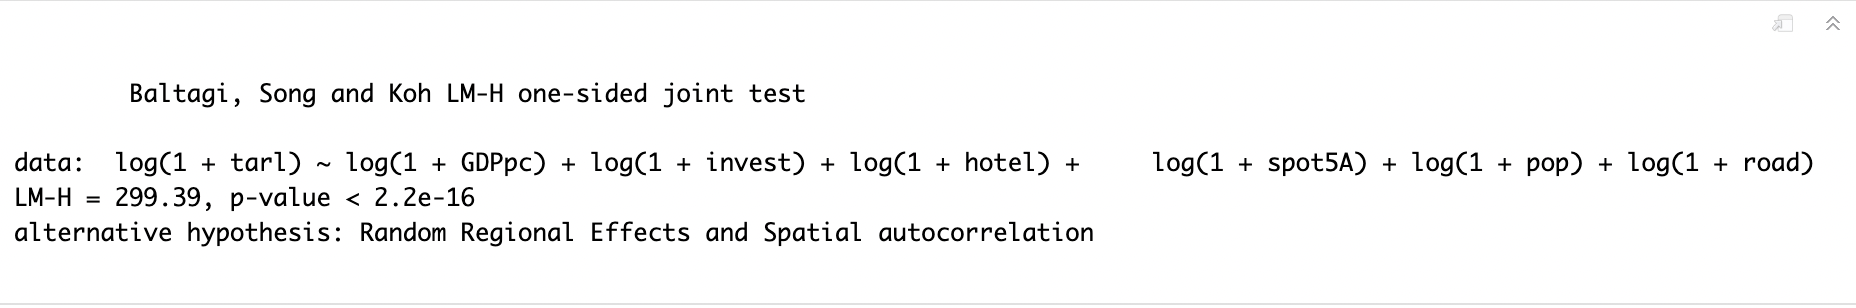
\includegraphics[scale=0.48]{lmtest1}}
	\caption{LM test for random effect and spatial autocorrelation}\label{F:lmtest1}
\end{figure}

$\bullet$ \textbf{$H_{0}:$ no spatial autocorrelation, allowing random effect}\par
We reject the null confidently. 
\begin{figure}[hbt]
	{\centering 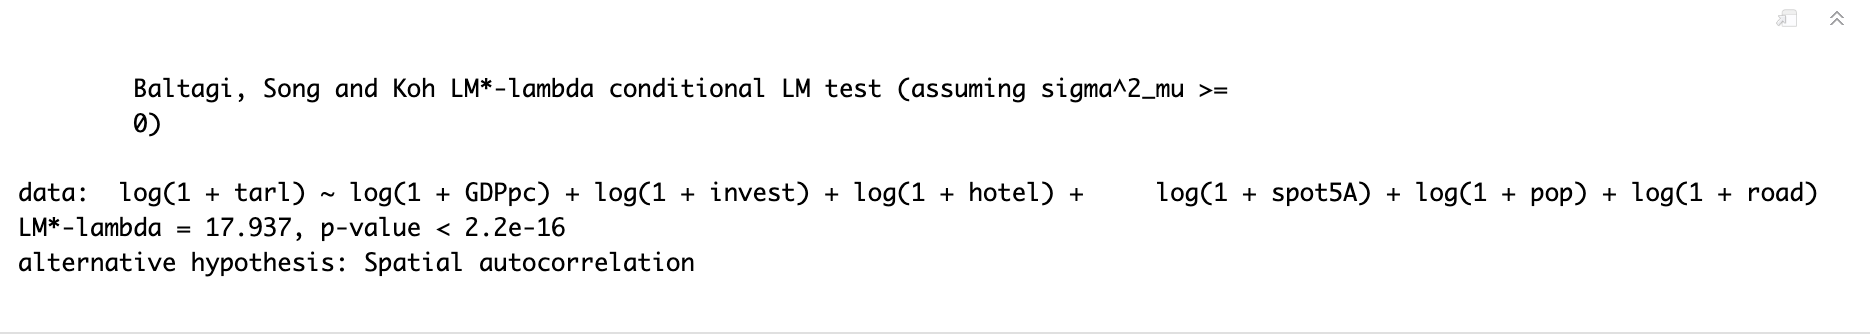
\includegraphics[scale=0.48]{lmtest2}}
	\caption{LM test for spatial autocorrelation}\label{F:lmtest2}
\end{figure}

$\bullet$ \textbf{$H_{0}:$ no random effect, allowing spatial autocorrelation}\par
We reject the null confidently. 
\begin{figure}[hbt]
	{\centering 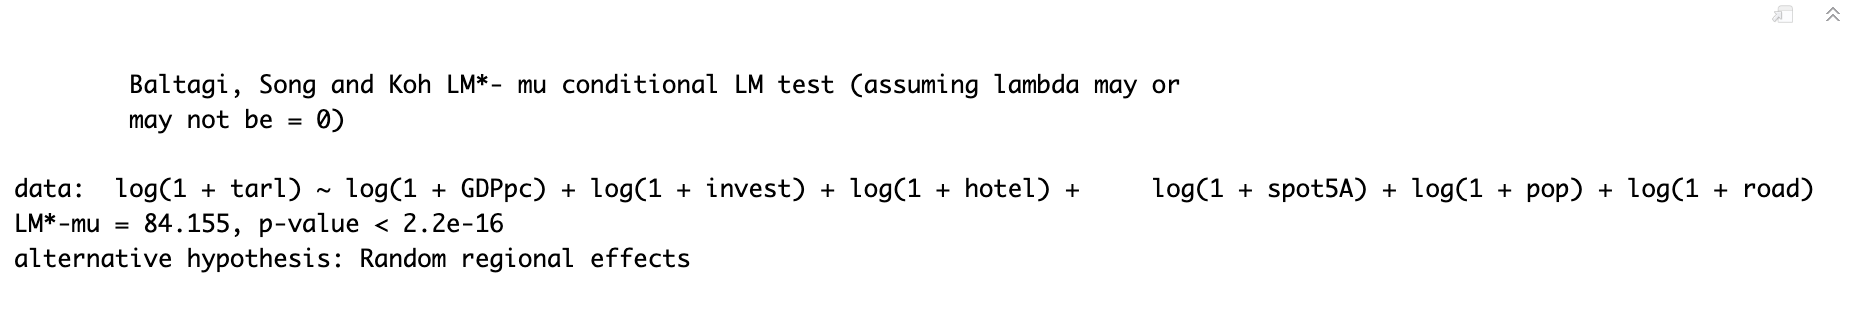
\includegraphics[scale=0.48]{lmtest3}}
	\caption{LM test for random effect}\label{F:lmtest3}
\end{figure}

\subsection{Test for  the appropriateness of fixed effect or random effect}\par\hfill

Hausman test tells us whether the fixed effects model or random effects model is more appropriate. In other words, whether the assumption of random effect is supported by the data. This is a spatial version of the traditional Hausman test.

$\bullet$ \textbf{ $H_{0}:$ The preferred model is Random Effect}
\begin{figure}[hbt]
	{\centering 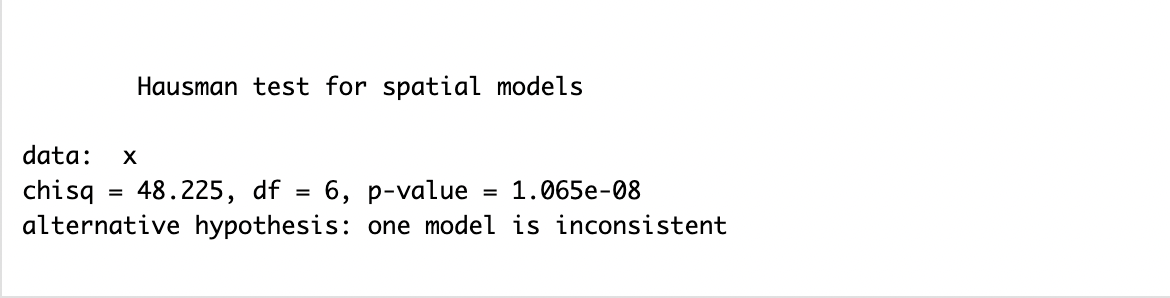
\includegraphics[scale=0.68]{hausman}}
	\caption{spatial Hausman test}\label{F:hausman}
\end{figure}

\subsection{Test for  the appropriateness of SAR or SAR error}\par\hfill

This is a locally robust LM tests for spatial lag (error) correlation in panel models. It is a panel version for the test developed by \href{https://www.sciencedirect.com/science/article/pii/0166046295021116}{Anselin et al. (1996)}. Our results are highly significant for both the spatial lag and the spatial error dependence. But the LM score is much higher for the spatial lag model ($1181.2$) than that for the error model ($255.03$). This might suggest that the spatial lag model is a better specification (or SARAR).

$\bullet$ \textbf{ $H_{0}:$ No spatial lag dependence}
\begin{figure}[hbt]
	{\centering 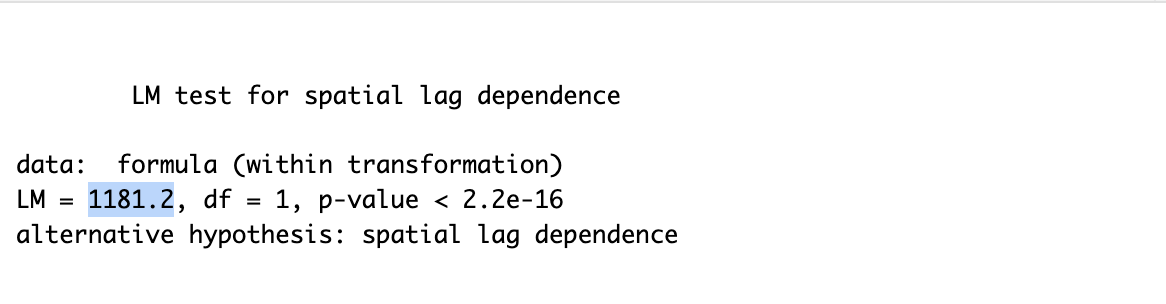
\includegraphics[scale=0.68]{lmlag}}
	\caption{LM test for spatial lag dependence in panel model}\label{F:lmlag}
\end{figure}

$\bullet$ \textbf{ $H_{0}:$ No spatial error dependence}
\begin{figure}[hbt]
	{\centering 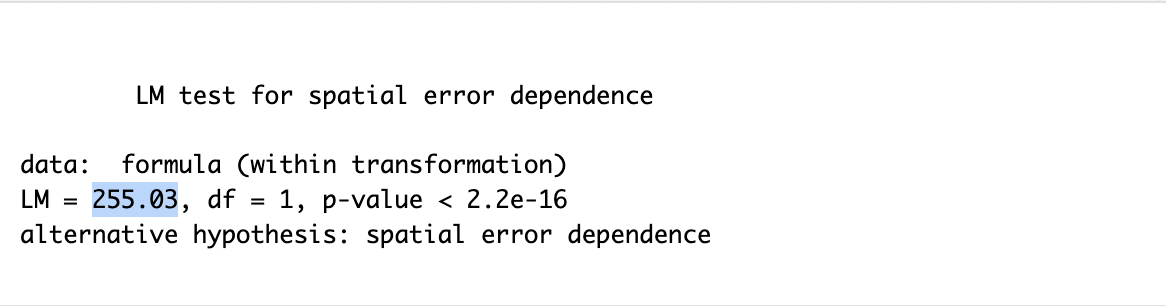
\includegraphics[scale=0.68]{lmerror}}
	\caption{LM test for spatial error dependence in panel model}\label{F:lmerror}
\end{figure}

\section{Panel spatial regressions}

I estimated the following spatial autoregressive panel regression model, with individual fixed effect.
\[ \begin{aligned}
	 \ln(1+tarl) &= \ln(1 + GDPpc) + pslry + \ln(1+invest) + \ln(1+hotel) + \ln(1+spot5A)+ \ln(1+scenum) \\
	 &+ \ln(1+pop) + \ln(1+bus) + \eta_{i} +\epsilon 
\end{aligned}
\]

Here, $pslry$ is the spatially lagged salary, and the other variables should be clear. The result is quite good.
\begin{figure}[hbt]
	{\centering 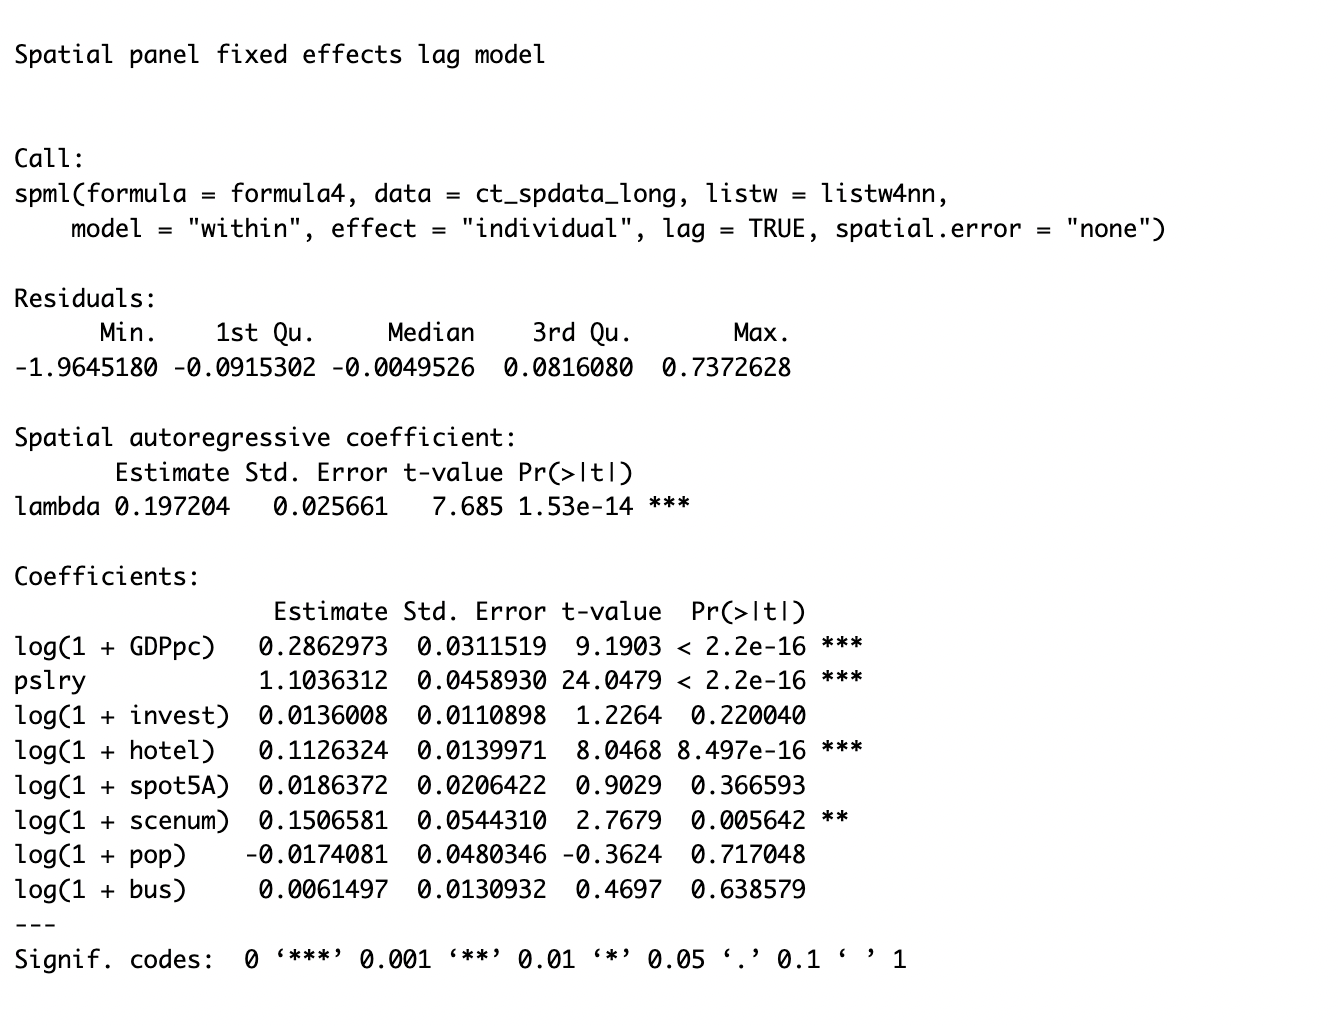
\includegraphics[scale=0.68]{lagfe}}
	\caption{Spatial autoregressive regression with individual fixed effect}\label{F:lagfe}
\end{figure}

But here is a strange thing: if we also include the spatial error (i.e., run the SARAR model), then we get two spatial parameters with the opposite signs, and they are about the same magnitude. I also added time fixed effect here.
\begin{figure}[hbt]
	{\centering 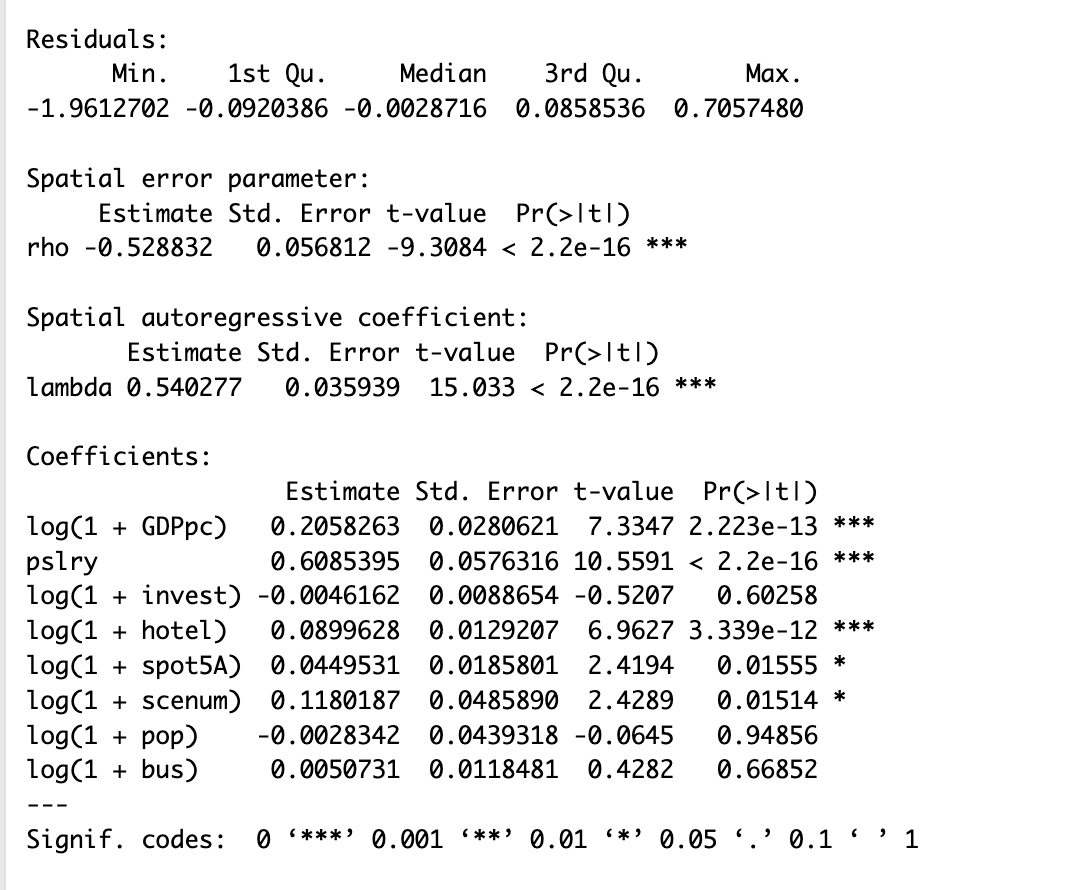
\includegraphics[scale=0.68]{sararfe}}
	\caption{SARAR regression with individual and time fixed effect}\label{F:sararfe}
\end{figure}

\newpage

\section{Two regime}

I followed this definition for our regimes.  So
\[	d_{it} = \begin{cases}
	1, &\text{if $y_{it} > \sum_{j = 1}^{N}y_{jt}$;}\\
	0, &\text{otherwise.}
\end{cases}	\]

I use total tourism arrivals for the dependent variable here. The result is as follows 

\begin{figure}[hbt]
	{\centering 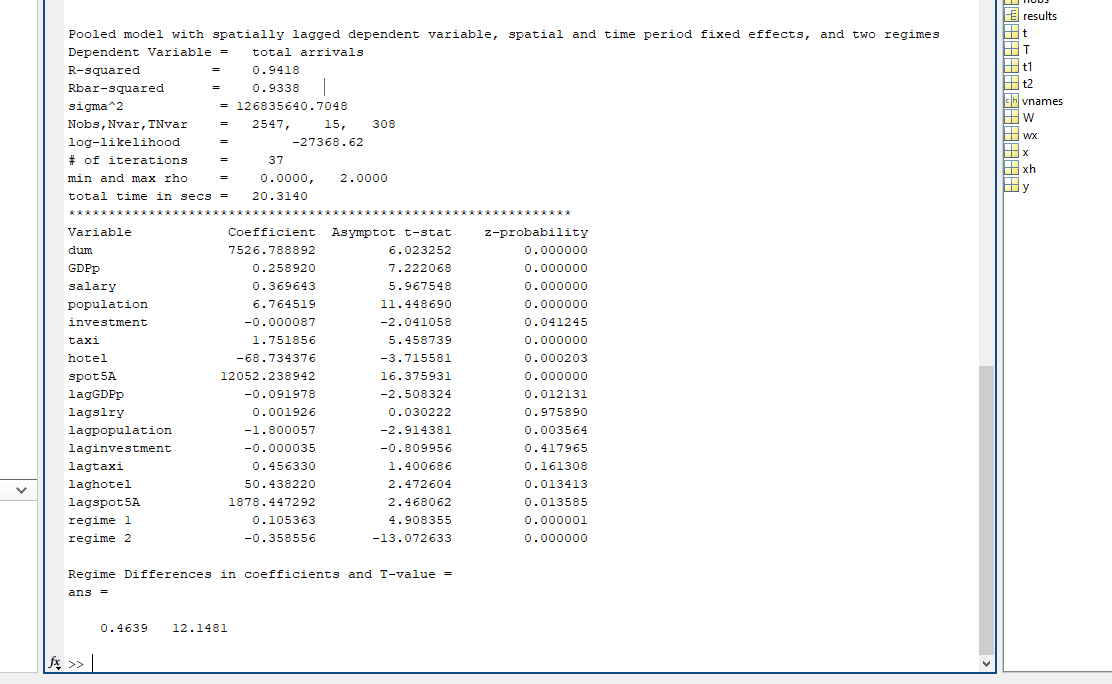
\includegraphics[scale=0.48]{/Users/jialiangchen/Documents/spmodeltoruism/results/two_regimes.png}}
	\caption{Two regime spatial Durbin model, with time and individual fixed effects}\label{F:2regimes}
\end{figure}

The $regime1$ (i.e., the strong cities) has a positive spatial effect, and the $regime2$ (i.e., the weak cities) has a much more negative effect. This is in aligned with our expectation.

\section{issues}
1. Panel version of Moran' I. There is a online reference about this. But he simply used the average of the cross-sectional Moran's I stats, and them claim that the resulting stat follows a normal distribution, and therefore can be used for test. This is problematic: it seems that he assumes serial independence. Some other versions exist in the literature, but we have to coded it from scratch (does it worth that)? 

2. I also have a combo of random variables including the average travel cost ($:= \text{total revenue}/\text{total arrivals}$). Based on my experiment, it will in general improve the fit to some extent.  Also, the coefficients are negative as should be, so it may not be suffering from severe endogeneity. 

3. I have not try other estimation methods (say, generalize methods of moments). This might be more important if we choose to include the average travel cost variable.

%\printbibliography %Prints bibliography
		
\end{document}
